\section{Real structures and their fixed three-spheres}\hypertarget{tag-02P9}{}\label{mapsI:real-forms}

We use the family marking
$\Lambda=\mathbb Z\langle\widehat\gamma,\widehat u,\widehat w,
\widehat\delta\rangle$ and its dual covector $\gamma$.
In this section $d=\widehat\delta$, $g=\widehat\gamma$,
$u=\widehat u$, and $w_{\Lambda}=\widehat w$; an unadorned $w$ in a
lattice expression denotes $w_{\Lambda}$, whereas the scalar parameter is
$w=\exp(-\pi i c)$. Put
\[
 e=\Pi_c d=(0,1)^t,\qquad E=d\otimes\gamma,
 \qquad \Pi_c=
 \begin{pmatrix}6\mu&\tau&1&0\\\beta^{\rm part}+c&\mu&0&1\end{pmatrix},
\]
\[
 D_c=\operatorname{Im}(\beta^{\rm part}+c)
       -6(\operatorname{Im}\mu)^2/\operatorname{Im}\tau<0.
\]
Thus $d$ is a lattice vector and $e$ is its image in the complex translation
space. The circle $\rho(s)$ is translation by $se$, $s\in\mathbb R/\mathbb Z$.
The clockwise root generators and the affine vectors are
\[
 A_1=\begin{pmatrix}1&0&0&0\\6&0&1&0\\-6&-1&-1&0\\-2&1&0&1\end{pmatrix},\quad
 A_2=\begin{pmatrix}1&0&0&0\\0&0&-1&0\\-6&1&0&0\\3&0&1&1\end{pmatrix},
\]
\[
 M_0=(A_1A_2)^{-1},\qquad
 v_1=(1,2,-4,0)^t,\qquad v_2=(-1,-3,3,0)^t.
\]
These are the same conventions as in the family construction. In cusp
coordinates $q=1/t$ and $s=(2\pi i)^{-1}\log q$, the bounded matrix $C_c(q)$
is defined by $Z_c=sB_0+C_c(q)$, with
$B_0=\left(\begin{smallmatrix}0&1\\-1&0\end{smallmatrix}\right)$.
In particular $\Pi_cg=(6\mu,-s+C_{c,21})^t$.
We write $D_1,D_2,D_{12}$ for the three cusp double curves belonging to
edges in directions $e_1,e_2,e_1-e_2$, respectively. Thus $D_2$ is the
fixed sphere of the circle action $\rho$, whereas $D_1$ is the double
curve along which the literal character has a limit. This distinction
is essential in the real calculation as well.

\begin{proposition}[Two conjugacy classes of real structures]\hypertarget{tag-02PE}{}\label{mapsI:src:A.3.1}
\StatementRecord{mapsI:src:A.3.1}{proved}{02PE}{\SeriesRef{fam:src:B.4.2}, \SeriesRef{fam:src:B.4.1}; \cite[Theorem~3.1, p.~48]{Illman1972}; \cite[Theorem 4.1(1)]{Knudson2004}}

For a real member the antiholomorphic involutions have exactly two
conjugacy classes under holomorphic automorphisms. For any fixed
involutive splitting $\sigma$ they are represented by $\sigma$ and
$\rho(1/2)\sigma$. Every nonempty fixed set is a closed connected
orientable totally real three-manifold with the mod-two homology of
$S^3$. The circle $\rho$ preserves each such fixed set and acts
semifreely on it.
\end{proposition}



\begin{proof}
\begin{enumerate}[label=\arabic*.,leftmargin=*]
\item The real comparison of Proposition~\ref{fam:src:B.4.2} has derivative complex conjugation in the
second period coordinate. It therefore conjugates translation by
$b\in\C/\Z$ to translation by $\bar b$. In multiplicative notation its
action is $z\mapsto1/\bar z$. The square of $z\sigma$ is $z/\bar z$,
so it is an involution exactly for $z\in\R^*$. Conjugation by $y\in\C^*$
changes this coefficient to $|y|^2z$, giving exactly its two signs.
The automorphism computation used here is Proposition~\ref{fam:src:B.4.1}: the integral centralizer has linear part $aI$, the cusp and
finite norm equations force $a=1$ for a self-map, and the global
translation sheaf has $H^0=\C e$ with integral periods $\Z e$.
These are precisely the three steps needed to identify the full group
with $\C^*$, rather than only its identity component.

\item At a fixed point an antiholomorphic involution has a real three-dimensional
fixed tangent space, and its complexification is the full tangent space.
An invariant metric and its exponential map identify its fixed locus
locally with this real subspace. It is therefore a closed totally real
three-manifold. The smooth $\mathbb Z/2$ action admits an equivariant
triangulation by \cite[Theorem~3.1, p.~48]{Illman1972}; compactness and finite
dimension give the finite-dimensional $G$-CW hypothesis. Smith's theorem,
in the form of
\cite[Theorem 4.1(1)]{Knudson2004}, applies to the smooth finite action on
the sphere and gives the stated mod-two homology. A nonempty
three-dimensional fixed set is consequently connected, and its first
mod-two cohomology vanishes; its orientation class $w_1$ therefore
vanishes. On the unit circle $1/\bar z=z$, so $\sigma$ commutes with
$\rho$. Its stabilizers are inherited from the checked semifree action
on $X$ and hence are either trivial or the whole circle.
\end{enumerate}
\end{proof}

We now fix a representative of each sign class, instead of leaving the
symbol $\sigma$ unspecified. Put
\[
 L_F=(2\pi i)^{-1}\log F,\qquad L_G=(2\pi i)^{-1}\log G,
 \qquad F^3=t,\quad G^4=t-1.
 \hypertarget{tag-02P4}{}\label{mapsI:real-eq-1}
\]
The roots are positive over $t>1$. We continue from that interval
through the upper half $t$-plane. Their logarithms are taken on the
orbifold uniformizing cover. Write $\iota$ for its reflection lift.
Every point of $-i\R_{>0}$ has a representative $c=1/2+iy$, and every
point of $i\R_{>0}$ has a representative $c=-1/2+iy$, with $y$ in the
admissible range. Set
\[
\begin{array}{c|c|c}
 &\alpha&S(t)\\\hline
 c=1/2+iy&1/3&2L_F-4L_G-1/6\\
 c=-1/2+iy&1/2&-2L_G+1/4
\end{array}
\qquad b_c(z)=\alpha\Pi_c(z)g+S(t(z))e.
\label{mapsI:real-eq-2}
\]

\begin{theorem}[Explicit real involutions and all fixed fibres]\hypertarget{tag-02PF}{}\label{mapsI:src:A.3.2}
\StatementRecord{mapsI:src:A.3.2}{proved}{02PF}{\SeriesRef{fam:src:B.4.2}, \SeriesRef{mapsI:real-eq-4}, \SeriesRef{mapsI:real-eq-2}, \SeriesRef{fam:src:A.3.1}, \SeriesRef{mapsI:real-eq-1}}

On the ordinary period charts the formulas
\[
 \sigma_c[z,\zeta]=[\iota z,\bar\zeta+b_c(\iota z)],
 \qquad \sigma_c^- =\rho(1/2)\sigma_c
 \label{mapsI:real-eq-3}
\]
extend to antiholomorphic involutions of the compact threefold.
With these representatives their complete fixed-set data are as follows.
Here $2T^2$ means the disjoint union of two real two-tori; every displayed
circle in a double curve avoids its two triple-point endpoints.
\begin{center}\small
\begin{tabular}{cclccc}
\toprule
$w$&involution&image in $\RP^1$&on $S_1$&on $S_2$&on $W$\\
\midrule
$-ir$, $r>0$&$\sigma_c$&all $\RP^1$&$2T^2$&$2T^2$&$T^2\sqcup S^1_{D_2}\sqcup S^1_{D_{12}}$\\
$-ir$, $r>0$&$\sigma_c^-$&$[1,\infty]$&$\varnothing$&$T^2$&$S^1_{D_1}\sqcup S^1_{D_2}$\\
$ir$, $r>0$&$\sigma_c$&$\varnothing$&$\varnothing$&$\varnothing$&$\varnothing$\\
$ir$, $r>0$&$\sigma_c^-$&$[\infty,1]$ through $0$&$2T^2$&$T^2$&$S^1_{D_1}\sqcup S^1_{D_{12}}$\\
\bottomrule
\end{tabular}
\end{center}
The first interval is the closure of $t>1$; the second is the closure
of $t<1$. On every open real arc contained in the indicated image the
real regular fibre is $2T^2$. No triple point is real for these structures.
\end{theorem}



\begin{proof}
\begin{enumerate}[label=\arabic*.,leftmargin=*]
\item We first verify the global map. Use the lattice reflection from Proposition~\ref{fam:src:B.4.2},
\[
 H=\begin{pmatrix}1&0&0&0\\0&1&0&0\\-6&0&-1&0\\0&-1&0&-1\end{pmatrix},
 \quad E=d\otimes\gamma,
 \quad\Pi_{-\bar c}(\iota z)H=-\overline{\Pi_c(z)}.
\]
The initial map $\zeta\mapsto-\bar\zeta$ has target affine vectors
$-\varepsilon+d$ and $\varepsilon'-3d$. The normalization from this
target at parameter $c_0=-\bar c$ to the canonical datum at $c_0+1$
has linear part $-I$ and translation
\[
 b^{\rm norm}_{c_0}=\tfrac13\Pi_{c_0}g+(2L_F-4L_G)e.
 \hypertarget{tag-02P5}{}\label{mapsI:real-eq-4}
\]
Its period defects at the two finite generators are
$(0,-2,2,0)^t$ and $(0,0,2,0)^t$. To check them, the logarithmic increments
are $-2/3$ and $1$, and one multiplies the two displayed matrices $A_j$
by $g/3$. The finite difference vectors in the complex translation space are $2e$ and $-4e$, so subtracting
their logarithmic collars leaves holomorphic translations on both full
root discs. At the cusp
$2L_F-4L_G=s/3-(2\pi i)^{-1}\log(1-q)$ and
$\Pi g=(6\mu,-s+C_{21})^t$. The logarithmic terms cancel and give the
holomorphic toric unit
$(2\mu,C_{21}/3-(2\pi i)^{-1}\log(1-q))$.
Thus \eqref{mapsI:real-eq-4} extends over all three fillings, with its inverse.

\item For $c=1/2+iy$ compose this normalization with the initial reflection
and then with the constant translation $e/6$. This gives exactly the
first line of \eqref{mapsI:real-eq-2}. For $c=-1/2+iy$, additionally close the parameter
shift by the following explicit even-shift formula with $h=-2$,
\[
 b_{h,c_0}=-\frac h{12}\Pi_{c_0}g+
 \left(h(L_F-L_G)-\frac{h^2}{24}\right)e.
\]
A final constant translation $-e/4$ gives the second line of \eqref{mapsI:real-eq-2}.
The displayed translation has integral affine defects on the ordinary cover, holomorphic finite-chart corrections, and a nonvanishing toric-unit expression at the cusp; it represents the even shift of Proposition~\ref{fam:src:A.3.1}. Its cusp expression is checked immediately below. Indeed put $\ell=L_F-L_G=-s/12+\kappa_0(q)$ and
$C_{c,21}(q)=c+C_{0,21}(q)$, and set
$D_0(q)=C_{0,21}(q)-12\kappa_0(q)$.
The explicit even-shift translation becomes
\[
 b_{h,c}=
 \left(-h\mu/2,-h(c+D_0)/12-h^2/24\right)^t.
\]
The logarithmic terms have cancelled exactly. Exponentiating both
coordinates gives holomorphic nonzero torus multipliers on the whole cusp
disc; multiplication by these units extends over every toric stratum.
Compatibility with the period deck group is the integral identity
$\exp(2\pi i h\lambda_1)=1$ for $h\in2\mathbb Z$ and
$\lambda_1\in\mathbb Z$. The finite-chart defects are checked by the
same displayed $A_j$ and root logarithms used for the normalization.

\item Over $t>1$ we have
$\Re\mu=1/2$, $\Re\tau=\Re\beta^{\rm part}=0$ and the logarithms in
\eqref{mapsI:real-eq-1} are purely imaginary. The two squares are respectively the
integral period translations $2\widehat w$ and $3\widehat w$.
The square is a holomorphic automorphism and is consequently the
identity everywhere. This proves the involution claim.

\item We next give exact equations for all real fibres. Put $a=\Re c$ and
$R=-H+2aE$. In the chosen branch the reflection identifications on
$t>1$, $0<t<1$, $t<0$ are respectively $1,g_2,g_0^{-1}$.
They follow by reflecting the chosen upper-half-plane paths; equivalently
the root arguments are $(0,0)$, $(0,\pi/4)$ and $(\pi/3,\pi/4)$.
The three fibre involution matrices are
\[
 R_>=R,\qquad R_m=A_2^{-1}R,\qquad R_<=M_0R.
 \hypertarget{tag-02P6}{}\label{mapsI:real-eq-5}
\]
In marked real coordinates let $r_c(t)=\Pi_c(t)^{-1}b_c(t)$,
where $\Pi_c^{-1}$ is the real inverse. The fixed tori are exactly
\[
 \{x\in\R^4/\Lambda:(I-R_\bullet)x=
                       r_c(t)+\epsilon d/2\pmod\Lambda\},
 \qquad\epsilon=0,1.
 \label{mapsI:real-eq-6}
\]
This specifies the cosets, including their parameter dependence. Their
identity subgroups are $T_{\langle w,d\rangle}$ on both outer arcs and
$T_{\langle u+w,d\rangle}$ on the middle arc. When nonempty there are
two cosets. Relative to any one solution their offsets are
$(g+u)/2$ on the right arc and $g/2$ on the other two arcs.

\item For completeness, the finite arithmetic deciding existence can be
performed without approximating the periods. An affine involution
$x\mapsto R_\bullet x+\beta$ has a fixed point if and only if its
square translation $(I+R_\bullet)\beta$ belongs to
$(I+R_\bullet)\Lambda$. In \eqref{mapsI:real-eq-2} the square translation is
\[
 (I+R_\bullet)\alpha g+2\Re S\,d.
\]
For $c=1/2+iy$ the values $2\Re S$ on the three arcs are
$-1/3,-4/3,-2/3$; for $c=-1/2+iy$ they are $1/2,0,0$.
The resulting integral square vectors are respectively
$(2w,0,2w)$ and $(3w,d,3w)$. Adding $d/2$ to the involution adds $d$
to each square vector. Taking column Hermite normal forms of
$I+R_\bullet$ gives exactly the nonempty entries in the table.
All three $I-R_\bullet$ have nonzero Smith factors $1,2$.
This proves the coset counts and offsets; the complete exact computation
is in \texttt{code/maps\_audit/MAPS/code/real\_involutions.py}. In particular the lift on
the left arc is $g_0^{-1}$, not $g_0$; the latter would give a nonintegral
square vector and is the wrong continuation convention.

\item At $t=0$ the root degree is odd. Conjugation by the degree-three deck
group acts transitively on the three reflection lifts; the centralizer
of a reflection in that deck group is trivial.
Thus the quotient has exactly the same two real tori as the adjacent
nonempty real regular fibres. In the empty cases there are none. This
also follows by solving the limiting affine equations, and checks the
full multiplicity-three quotient rather than treating it as a reduced
unramified fibre.

\item At $t=1$ write the affine deck map as
$G(x)=A_2x+v_2/4$. The real root involution has matrix $R_>$ and
translation
\[
 b_-=(1/3,0,0,-1/6)^t,
 \qquad b_+=(1/2,0,0,1/4)^t
\]
for the two parameter signs. The real locus of the quotient is the
quotient of the fixed sets of $G^kh$, $0\leq k<4$. Its even and odd
lift parities are identified internally by $G$, while $G^2$ preserves
each parity. Direct integer congruences show that the nonempty lift
parities are: both for negative $w$ and $\epsilon=0$; only even for
negative $w$ and $\epsilon=1$; neither for positive $w$ and $\epsilon=0$;
only odd for positive $w$ and $\epsilon=1$. Every nonempty lift has
two tori, exchanged by $G^2$. Each parity therefore contributes one
torus downstairs, not a Klein bottle. The exhaustive congruence check
\texttt{code/maps\_audit/MAPS/code/real\_finite\_four.py} uses denominator $24$: translation
denominators divide $12$, and the nonzero Smith factors are $1,2$, so
every component has such a representative. It checks the component
permutation, not just the dimension of the fixed eigenspace. The normal
real line has fourth power of sign positive for the even parity and
negative for the odd parity. This establishes the two one-sided
endpoints at $t=1$ recorded in the table.

\item It remains to compute the cusp, which also excludes hidden real
components confined to a singular fibre. Put
$A=C_{12}(0)$; the cusp normalization gives
\[
 \Re\mu(0)=1/2,\quad A\in i\R,\quad C_{21}(0)=c-A,
 \quad C_{11}(0)=6\mu(0),\quad C_{22}(0)=\mu(0).
\]
In a toric lift the involution is
$x\mapsto U/\bar x$, with
\[
\begin{array}{c|cc}
 &b_1(0)&b_2(0)\\\hline
 w=-ir&2\mu(0)&C_{21}(0)/3-1/6\\
 w=ir&3\mu(0)&C_{21}(0)/2+1/4
\end{array}
\qquad U_j=e^{2\pi i b_j(0)}.
\hypertarget{tag-02P7}{}\label{mapsI:real-eq-7}
\]
Thus $U_2>0$ in both rows, whereas $U_1>0$ in the first and $U_1<0$
in the second. Replacing $\sigma_c$ by $\sigma_c^-$ negates $U_2$.
The smooth central orbit has a real torus precisely when both units
are positive, with equations $|x_j|^2=U_j$.

\item For an edge $v$, set $n=(-v_2,v_1)^t$. The period translate bringing
the inverted edge back is $B_0n=v$. Its curve coordinate $z=x^n$ has
involution
\[
 z\longmapsto K_v/\bar z,
 \qquad K_v=U^n e^{2\pi i n^tC(0)n}.
 \hypertarget{tag-02P8}{}\label{mapsI:real-eq-8}
\]
The signs for $(D_1,D_2,D_{12})$ are $(-,+,+)$ for negative $w$
and $(-,-,-)$ for positive $w$. Negating $U_2$ reverses the first and
third signs, but not the second. A positive sign gives the single
circle $|z|^2=K_v$; a negative sign gives no fixed point. Central
inversion exchanges the two triangle classes of the periodic fan, so
it exchanges the two triple points. These calculations prove every
cusp entry. Finally a nonempty fixed three-manifold cannot be confined
to the special fibres: a holomorphic function constant on an open
piece of a totally real submanifold is locally constant. This also
proves that the positive-$w$ representative with no regular real
fibres is entirely fixed-point free.
\end{enumerate}
\end{proof}

\begin{theorem}[The real three-manifolds]\hypertarget{tag-02PG}{}\label{mapsI:src:A.3.3}
\StatementRecord{mapsI:src:A.3.3}{proved}{02PG}{\SeriesRef{mapsI:src:A.3.2}}

Every nonempty fixed set in Theorem~\ref{mapsI:src:A.3.2} is diffeomorphic to $S^3$.
Its fundamental group is trivial and its integral homology is
$(\Z,0,0,\Z)$. For negative imaginary $w$, the restricted circle action
is the standard semifree action on $S^3$ with fixed circle
$D_2^{\sigma_c}$. For positive imaginary $w$, the nonempty real form
has a free circle action isomorphic, up to circle and orientation
conventions, to the Hopf action.
\end{theorem}



\begin{proof}
\begin{enumerate}[label=\arabic*.,leftmargin=*]
\item For negative imaginary $w$ both fixed manifolds meet $D_2$ in one circle.
Their circle action is semifree, so the orbit space is a compact
orientable surface with boundary. The local quotient at a fixed circle
is the quotient of $S^1\times\C$ by scalar rotation on $\C$, hence is
a boundary collar. Over the surface interior the principal circle bundle
is trivial because the surface has boundary and $H^2=0$. Changes of
boundary trivialization extend over the attached normal discs by
rotation. Thus the three-manifold is
\[
 (B\times S^1)\ \cup_{\partial B\times S^1}\ (\partial B\times D^2).
\]
If $B$ has genus $g_B$ and $b_B$ boundary components, van Kampen or its
surface handle decomposition gives first homology
$\Z^{2g_B+b_B-1}$. Smith's theorem makes this rank zero. Since $b_B>0$,
we have $g_B=0,b_B=1$. The displayed manifold is then
$\partial(D^2\times D^2)=S^3$, with the indicated circle action. This
derives the smooth recognition from an explicit surface decomposition.

\item For positive imaginary $w$ the nonempty real manifold is free under
$\rho$. The two real tori on $t<1$ join at the single real torus over
$1$. At $0$ the odd root comparison is a torus product. At infinity
they are capped by the real neighbourhoods of $D_1$ and $D_{12}$.
These are solid tori: the primitive circle in the edge direction
collapses and the remaining real circle is their core. In the outer
real-fibre lattice $\Z\langle w,d\rangle$ the two cap meridians are
$w$ and $w-d$.

\item We check the intervening torus identification. Put
$B_1=A_2^{-1}A_1^{-1}A_2$ and $C=B_1^2$. The two real-arc involutions
satisfy $R_<R_m=B_1$, $R_mB_1R_m=B_1^{-1}$ and $B_1^3=I$.
Moving between the real root lifts requires
$B_1^kR_mB_1^{-k}=B_1R_m$, so $2k\equiv1\pmod3$ and $k=2$.
Thus the actual odd-root transport is $C$, not merely an arbitrary
matrix conjugating the two reflections. It satisfies $R_<=CR_mC^{-1}$, and
$C(u+w)=-w+d$. The exchange across the multiplicity-four real torus
is $A_2^2$; after this odd-root transport it is
$CA_2^2C^{-1}$, whose restriction to $\langle w,d\rangle$ is
$w\mapsto-w$, $d\mapsto d$. Consequently the meridians, compared on
one boundary torus, have determinant of absolute value one. The
resulting genus-one Heegaard splitting is $S^3$: primitive meridians
intersecting once can be taken to the two coordinate circles by an
integral torus automorphism, giving the usual two solid tori of $S^3$.
The free circle $d$ then has Euler number of absolute value one, so
the displayed bundle over $S^2$ is the Hopf bundle. This proves the
integral assertions, beyond the mod-two information.
\end{enumerate}
\end{proof}

\begin{proposition}[Restrictions of the repaired circle quotient]\hypertarget{tag-02PH}{}\label{mapsI:src:A.3.4}
\StatementRecord{mapsI:src:A.3.4}{proved}{02PH}{\SeriesRef{mapsI:src:A.2.1}, \SeriesRef{mapsI:real-eq-2}}

The repaired map $e_{\rm q}$ of Theorem~\ref{mapsI:src:A.2.1} may be chosen $\rho$-invariant. Its restriction to
every nonempty real form is null-homotopic. On an ordinary real fibre
its image consists of the two quotient-circle values
\[
 \theta=\tfrac12\gamma(r_c(t)),\qquad
 \theta=\tfrac12\gamma(r_c(t))+\tfrac12\pmod\Z,
 \quad
 \gamma(r_c(t))=\alpha+\frac{\Im S(t)}{D_c(t)},
 \label{mapsI:real-eq-9}
\]
with $\alpha,S$ from \eqref{mapsI:real-eq-2}. The circle action is along each real
two-torus and is annihilated by $e_{\rm q}$.
\end{proposition}



\begin{proof}
\begin{enumerate}[label=\arabic*.,leftmargin=*]
\item The literal quotient is circle invariant. In a cusp extension
$\theta':N_0\to S^1$, each orbit circle has degree zero: its class is
$d$, which vanishes in $\pi_1(N_0)$. The quotients
$\theta'(\rho(s)x)/\theta'(x)$ therefore have a continuous real lift
vanishing at $s=0$ and periodic in $s$. Averaging this real lift over
$s\in\R/\Z$ changes $\theta'$ to a circle-invariant map. The cocycle
identity proves invariance, and on an invariant outer collar the lift
is zero, so the replacement agrees exactly with the prescribed map.
The same construction is smooth. Thus $e_{\rm q}|_{\operatorname{Fix}\sigma}$
factors through its circle orbit space, which is $D^2$ or $S^2$ by the
preceding proof. Both have only two-dimensional homotopy type and
$S^3$ is two-connected, so this restriction is null-homotopic.
The first row of $I-R_\bullet$ is $(2,0,0,0)$, giving the two values
in \eqref{mapsI:real-eq-9}. The real inverse of the period matrix sends $S e$ to
first coordinate $\Im S/D_c$; this follows by subtracting
$(\Im\mu/\Im\tau)$ times its first imaginary-coordinate equation
from the second. Both real-fibre identity subgroups have zero
$\gamma$-coordinate, proving the remaining assertions.
\end{enumerate}
\end{proof}

The formulas specify the embedded fixed sets by their torus cosets and
their actual finite and toric attachments. No ambient-isotopy
classification or value of the Haefliger knot invariant of these
embedded three-spheres is asserted here.


\begin{cited}[The coherent closing translation]\hypertarget{tag-0322}{}\label{push:src:C.3.5}
\StatementRecord{push:src:C.3.5}{proved}{0322}{\SeriesRef{fam:src:A.3.1}; \citet[Proposition~7.8, pp.~91--92, and Proposition~C.2, p.~102]{DuEtAl2026v1}}

Fix the standard twists and the root and cusp markings of Proposition~\ref{fam:src:A.3.1}.
There is a coherent choice of the even-shift maps
\(\widetilde F_{h,c}:X_c\to X_{c+h}\), \(h\in2\mathbb Z\),
with the following explicit ordinary-chart translation. Choose global
roots \(F^3=t\), \(G^4=t-1\) on the uniformizing cover and put
\(\ell=(2\pi i)^{-1}\log(F/G)\pmod{\mathbb Z}\), \(e=(0,1)^t\).
Then the translation is
\begin{equation}\hypertarget{tag-02OP}{}\label{mapsI:closing:eq:C-explicit-closing}
 b_{h,c}=-\frac h{12}\Pi_c\widehat\gamma
              +\left(h\ell-\frac{h^2}{24}\right)e.
\end{equation}
For \(h=12\), it is the scalar multiplication
\begin{equation}\hypertarget{tag-02OQ}{}\label{mapsI:closing:eq:C-twelve-scalar}
 K(t)=\frac{t^4}{(t-1)^3}
\end{equation}
on the ordinary \(\mathbb C^*\)-coordinate, after removing an integral
period. On the finite root charts its scalar representatives are
\(K(t)s_1^{-12}\) and \(K(t)s_2^{12}\), respectively, both units.
In a cusp coordinate \(q=t_c\), the scalar representative is
\(q^{-1}H(q)\), with \(H\) a holomorphic nonvanishing function.
The same map has a holomorphic \((\mathbb C^*)^2\)-unit representative
on the entire cusp filling. These two representatives differ by
exactly the \(\widehat\gamma\) cusp deck transformation.

For six positive \(w\)-loops the closing map is
\(\widetilde F_{12,c_0-12}\); thus the stated cusp exponent is \(-1\)
with $w=e^{-\pi i c}$ and positive loops in the $w$-plane. This computes the closing
cocycle, not the mapping class of its composition with parallel
transport. In particular it does not imply \(6[\Phi]=0\).
\end{cited}
The expanded source derivation is retained in the proof compendium, Paper~I, label \nolinkurl{push:src:C.3.5}.




The raw even-shift formula and its coherent correction are due to \citet[Proposition~7.8, pp.~91--92, and Proposition~C.2, p.~102]{DuEtAl2026v1}. A complete re-derivation is given in \CompendiumRef{I}{app:rederive:push-src-C.3.5}.




\begin{figure}[htbp]
\centering
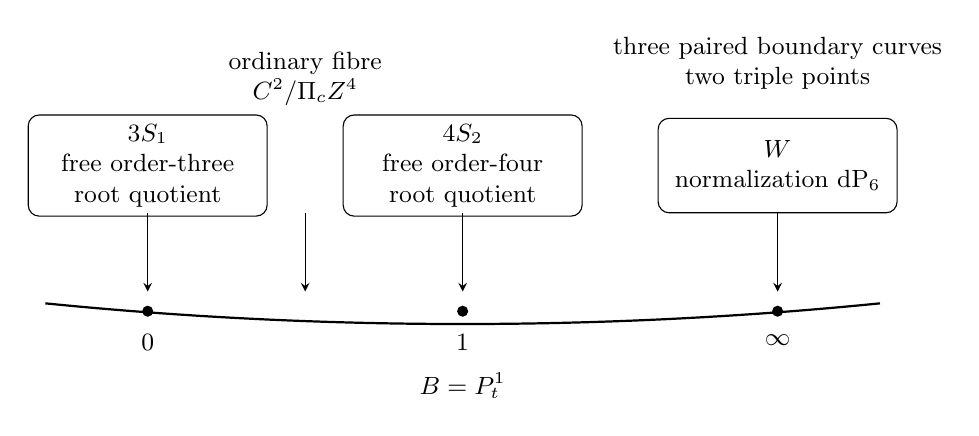
\begin{tikzpicture}[x=1cm,y=1cm,>=stealth,font=\small]
\draw[thick] (-5.3,0) .. controls (-1.8,-.35) and (1.8,-.35) .. (5.3,0);
\node at (0,-1.05) {$B=\mathbb P^1_t$};
\foreach \x/\lab in {-4/0,0/1,4/\infty}{
 \fill (\x,-.1) circle (2pt);
 \node[below=5pt] at (\x,-.1) {$\lab$};
 \draw[->] (\x,1.15)--(\x,.15);
}
\node[draw,rounded corners,align=center,text width=2.8cm,minimum height=1.2cm] at (-4,1.75)
 {$3S_1$\\free order-three\\root quotient};
\node[draw,rounded corners,align=center,text width=2.8cm,minimum height=1.2cm] at (0,1.75)
 {$4S_2$\\free order-four\\root quotient};
\node[draw,rounded corners,align=center,text width=2.8cm,minimum height=1.2cm] at (4,1.75)
 {$W$\\normalization $\mathrm{dP}_6$};
\draw[->] (-2,1.15)--(-2,.15);
\node[align=center] at (-2,2.85) {ordinary fibre\\$\mathbb C^2/\Pi_c\mathbb Z^4$};
\node[align=center] at (4,3.05) {three paired boundary curves\\two triple points};
\end{tikzpicture}
\caption{The fixed $(3,4,\infty)$ base data. The arrows denote the
restriction of $f$ to each indicated fibre, with its scheme
multiplicity retained. The ordinary period quotient, finite affine
quotients and the paired hexagon are the three actual local models
in the common conventions; their overlap maps are fixed there.}
\hypertarget{tag-01RL}{}\label{fig:I:orbifold}
\end{figure}

\begin{figure}[htbp]
\centering
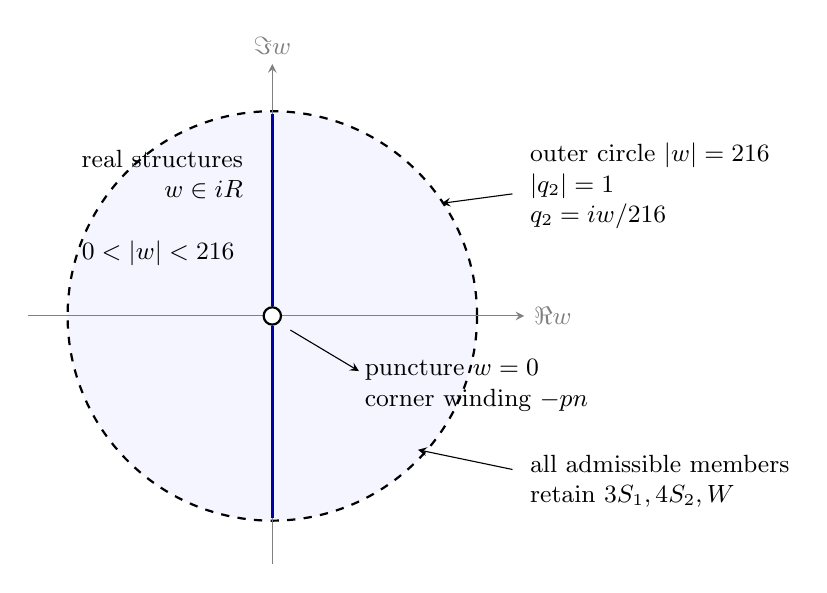
\begin{tikzpicture}[x=1cm,y=1cm,>=stealth,font=\small]
\fill[blue!4] (0,0) circle (2.6);
\draw[thick,dashed] (0,0) circle (2.6);
\draw[->,gray] (-3.1,0)--(3.2,0) node[right] {$\Re w$};
\draw[->,gray] (0,-3.15)--(0,3.2) node[above] {$\Im w$};
\draw[very thick,blue!65!black] (0,-2.56)--(0,-.13);
\draw[very thick,blue!65!black] (0,.13)--(0,2.56);
\fill[white] (0,0) circle (.11);
\draw[thick] (0,0) circle (.11);
\draw[->] (.23,-.18)--(1.1,-.7);
\node[anchor=west,align=left] at (1.05,-.88) {puncture $w=0$\\corner winding $-pn$};
\node[align=center] at (-1.45,.8) {$0<|w|<216$};
\node[anchor=west,align=left] at (3.15,1.65)
 {outer circle $|w|=216$\\$|q_2|=1$\\$q_2=iw/216$};
\draw[->] (3.05,1.55)--(2.15,1.43);
\node[anchor=east,align=right] at (-.25,1.8)
 {real structures\\$w\in i\mathbb R$};
\node[anchor=west,align=left] at (3.15,-2.1)
 {all admissible members\\retain $3S_1,4S_2,W$};
\draw[->] (3.05,-1.95)--(1.85,-1.7);
\end{tikzpicture}
\caption{The exact parameter disc for the standard fixed data.
The coordinate map is $w=e^{-\pi i c}$ and the coarser coordinate
map is $u=w^2$. The imaginary diameter is the fixed locus of
$w\mapsto-\bar w$, which is the reflected-family map.
The two boundary obstructions use the meridian comparison at the
puncture and the intrinsic Albanese nome at the outer circle.
The special fibres are over $t=0,1,\infty$ in every member, as
indicated in Figure~\ref{fig:I:orbifold}.}
\hypertarget{tag-01RM}{}\label{fig:I:parameter-disc}
\end{figure}

\begin{figure}[htbp]
\centering
\begin{tikzpicture}[x=1cm,y=1cm,>=stealth,font=\small]
\begin{scope}[shift={(-3.3,0)}]
 \fill[blue!5] (-1,0)--(-1,2.8)--(1,2.8)--(1,0)
  arc[start angle=30,end angle=150,radius=1.1547];
 \draw[thick] (-1,0)--(-1,2.8);
 \draw[thick] (1,0)--(1,2.8);
 \draw[thick] (1,0) arc[start angle=30,end angle=150,radius=1.1547];
 \node at (0,1.3) {$\mathcal F$};
 \node[align=center] at (0,-1.05)
 {$|\Re\tau|\le\tfrac12,\ |\tau|\ge1$\\$0\le\theta<\pi$};
 \draw[->] (0,2.1)--(0,3.1) node[above] {cusp};
\end{scope}
\begin{scope}[shift={(1.0,.2)},x={(1.8cm,0cm)},y={(.75cm,.5cm)},z={(0cm,2.2cm)}]
 \fill[blue!4] (0,0,0)--(1,0,0)--(1,0,1)--(0,0,1)--cycle;
 \draw[thick] (0,0,0)--(1,0,0)--(1,1,0)--(1,1,1)--(0,1,1)--(0,0,1)--cycle;
 \draw[thick] (1,0,0)--(1,0,1)--(0,0,1);
 \draw[thick] (1,0,1)--(1,1,1);
 \draw[dashed] (0,0,0)--(0,1,0)--(1,1,0);
 \draw[dashed] (0,1,0)--(0,1,1);
 \node[below] at (.5,0,0) {$0\le x_1<1$};
 \node[right] at (1,.5,0) {$0\le x_2<1$};
 \node[left] at (0,0,.5) {$0\le t<12$};
\end{scope}
\node[align=center] at (1.95,-1.55)
 {$U:\ t\mapsto t-6-6x_2$\qquad
  $V:\ t\mapsto t-6+6x_1$\\
  $Z:\ t\mapsto t+12$};
\end{tikzpicture}
\caption{A fundamental set for the index-twelve monodromy kernel
in the real parabolic stabilizer of $d$.
The base is a modular fundamental set with its rotation coordinate;
the fibre is the indicated Heisenberg parallelepiped. The displayed
face maps include the central shears. The representative map and
the boundary identifications are proved in
\ref{I:monodromy-fundamental-set}; the index twelve occurs in the
central fibre coordinate.}
\hypertarget{tag-01RK}{}\label{fig:I:monodromy-domain}
\end{figure}

\begin{proposition}[The fundamental set of the monodromy kernel]
\hypertarget{tag-0001}{}\label{I:monodromy-fundamental-set}
\StatementRecord{I:monodromy-fundamental-set}{proved}{0001}{\SeriesRef{fam:src:F.1.1}, \SeriesRef{fam:src:F.1.2}}
In the real coordinates $g(B,x,t)$ of
\ref{fam:src:F.1.1}, a measurable fundamental set for
$\Gamma\backslash P_d(\mathbb R)$ consists of the matrices
\[
 g(B,x,t),\qquad
 B=n(\Re\tau)a(\Im\tau)k(\theta),\quad
 \tau\in\mathcal F,\quad 0\le\theta<\pi,
 \quad x_1,x_2\in[0,1),\quad t\in[0,12).
\]
Here
$n(u)=\left(\begin{smallmatrix}1&u\\0&1\end{smallmatrix}\right)$,
$a(v)=\operatorname{diag}(\sqrt v,1/\sqrt v)$,
and $k(\theta)$ is the rotation matrix. Paired modular edges
are assigned to one side, and their lower-dimensional
stabilizer identifications use the corresponding lifts in
$\Gamma$: for
$S=\left(\begin{smallmatrix}0&-1\\1&0\end{smallmatrix}\right)$
and $T=\left(\begin{smallmatrix}1&1\\0&1\end{smallmatrix}\right)$,
we use $\widetilde S=g(S,0,9)$,
$\widetilde T=g(T,0,1)$ and
$\widetilde{-I}=g(-I,0,6)$.
Their maps on the three coordinates are
$(B,x,t)\mapsto(AB,Ax,t+\alpha(A))$, with
$\alpha(S)=9$, $\alpha(T)=1$ and $\alpha(-I)=6$.
The Heisenberg face identifications are the
maps printed in Figure~\ref{fig:I:monodromy-domain}.
\end{proposition}
\begin{proof}
\begin{enumerate}[label=\arabic*.,leftmargin=*]
\item The projection $g(B,x,t)\mapsto B$ maps $\Gamma$
onto $\operatorname{SL}_2(\mathbb Z)$ by
\ref{fam:src:F.1.1}. For any $B\in\operatorname{SL}_2(\mathbb R)$,
the usual modular reduction gives an integral matrix $A$
with $AB=n(u)a(v)k(\theta)$ in the stated set. Choose an
actual lift $g(A,y,s)\in\Gamma$ and multiply on the left.
For the displayed edge generators, the character formula
$\chi(g(A,0,t))=t-\alpha(A)\pmod {12}$ proves that the
three specified lifts lie in $\Gamma$. Substitution in
the group law gives each displayed coordinate map.
This is the specified map from a general parabolic element
to one over the modular set.
\item Two choices of lift over the same $A$ differ by
$\Gamma\cap H$. The group calculation in
\ref{fam:src:F.1.1} identifies this kernel with
$\langle U,V,Z\rangle$, where
$U=g(I,(1,0),-6)$, $V=g(I,(0,1),-6)$ and
$Z=g(I,0,12)$.
\item The multiplication law sends $(x,t)$ under $U$
to $(x+(1,0),t-6-6x_2)$, and under $V$ to
$(x+(0,1),t-6+6x_1)$. Powers of these maps first put
$x_1$ and $x_2$ in $[0,1)$. A power of $Z$ then puts
$t$ in $[0,12)$. All three are actual left translations
in $\Gamma$, so they retain the original coset.
\item Within the interiors of these intervals equality
of two reduced representatives forces their kernel
element to have zero $x$-translation and then zero
central translation. Modular uniqueness gives the same
conclusion in the base interior. The usual edge and
elliptic identifications, lifted by the specified
surjection, account for the measure-zero boundary.
This proves the fundamental-set assertion and all
displayed Heisenberg identifications.
\end{enumerate}
\end{proof}

